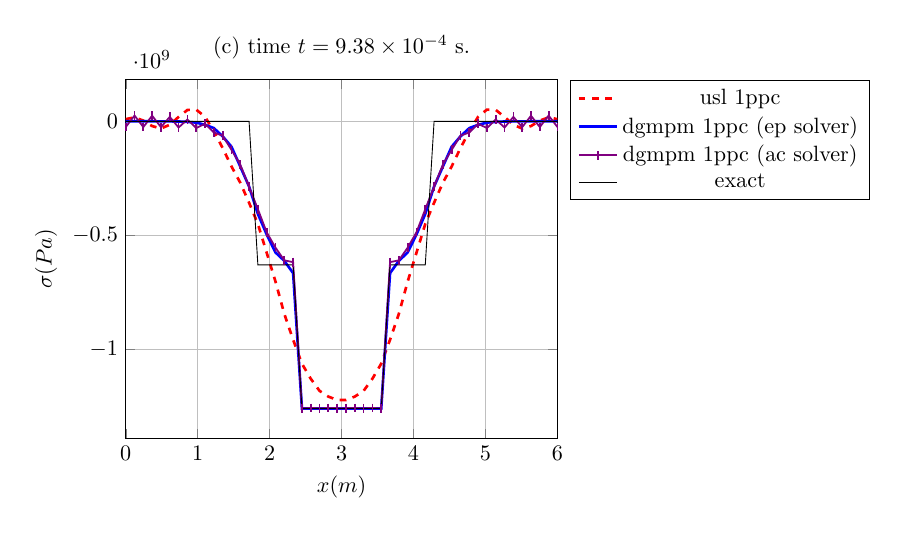
\begin{tikzpicture}[scale=0.8]
\begin{axis}[xlabel=$x (m)$,ylabel=$\sigma (Pa)$,ymajorgrids=true,xmajorgrids=true,legend pos=outer north east,title={(c) time $t = 9.38\times 10^{-4} $ s.},xmin=0.,xmax=6.]
\addplot[Red,very thick,mark=none,dashed] coordinates {(0.0,9503357.913254393) (0.12244897959183673,17431317.706177793) (0.24489795918367346,3141964.2004070086) (0.36734693877551017,-20870936.334975213) (0.4897959183673469,-31729533.500964552) (0.6122448979591837,-15041619.356117994) (0.7346938775510203,19157394.048619747) (0.8571428571428571,49883117.073489726) (0.9795918367346939,51435923.73285633) (1.1020408163265305,20122417.88732481) (1.2244897959183674,-44056112.68919331) (1.346938775510204,-116959231.47904712) (1.4693877551020407,-197881239.10650313) (1.5918367346938775,-269469505.4567269) (1.7142857142857142,-357548776.38031733) (1.836734693877551,-450600351.24984825) (1.9591836734693877,-577253338.2206764) (2.0816326530612246,-703619286.5327214) (2.204081632653061,-845658340.9284383) (2.326530612244898,-958996977.7445623) (2.4489795918367347,-1064208678.9122326) (2.571428571428571,-1130241655.9194942) (2.693877551020408,-1183692616.5567749) (2.816326530612245,-1208788567.6983013) (2.9387755102040813,-1223720874.1257663) (3.061224489795918,-1223720874.1257653) (3.183673469387755,-1208788567.6983027) (3.306122448979592,-1183692616.5567737) (3.4285714285714284,-1130241655.919495) (3.5510204081632653,-1064208678.9122312) (3.673469387755102,-958996977.7445619) (3.7959183673469385,-845658340.928436) (3.9183673469387754,-703619286.5327208) (4.040816326530612,-577253338.2206743) (4.163265306122449,-450600351.2498487) (4.285714285714286,-357548776.3803165) (4.408163265306122,-269469505.4567268) (4.530612244897959,-197881239.1065032) (4.653061224489796,-116959231.47904658) (4.775510204081632,-44056112.68919301) (4.8979591836734695,20122417.887324095) (5.020408163265306,51435923.7328558) (5.142857142857142,49883117.07348859) (5.26530612244898,19157394.04861957) (5.387755102040816,-15041619.356118202) (5.5102040816326525,-31729533.500964552) (5.63265306122449,-20870936.33497496) (5.755102040816326,3141964.2004074357) (5.877551020408163,17431317.70617821) (6.0,9503357.913254581) };
\addplot[Blue,very thick,mark=none,solid] coordinates {(0.0,-288.000337932026) (0.12244897959183673,-2340.8049612902105) (0.24489795918367346,-6717.6736351549625) (0.36734693877551017,-31436.18543893099) (0.4897959183673469,-82819.9714218378) (0.6122448979591837,-326370.9123286009) (0.7346938775510203,-787154.078435719) (0.8571428571428571,-2592039.5752673745) (0.9795918367346939,-5646941.091449976) (1.1020408163265305,-15363721.703147352) (1.2244897959183674,-29743749.637923777) (1.346938775510204,-65953645.19968498) (1.4693877551020407,-111309952.15841854) (1.5918367346938775,-198327314.7707913) (1.7142857142857142,-286130814.5665431) (1.836734693877551,-406728211.7590317) (1.9591836734693877,-496866659.92587715) (2.0816326530612246,-575814412.3291717) (2.204081632653061,-612581021.5556204) (2.326530612244898,-666589640.9783571) (2.4489795918367347,-1261004576.260559) (2.571428571428571,-1261004576.2605588) (2.693877551020408,-1261004576.2605588) (2.816326530612245,-1261004576.260559) (2.9387755102040813,-1261004576.260559) (3.061224489795918,-1261004576.2605588) (3.183673469387755,-1261004576.2605588) (3.306122448979592,-1261004576.2605586) (3.4285714285714284,-1261004576.260559) (3.5510204081632653,-1261004576.2605588) (3.673469387755102,-666589640.9783564) (3.7959183673469385,-612581021.5556185) (3.9183673469387754,-575814412.3291717) (4.040816326530612,-496866659.92587644) (4.163265306122449,-406728211.7590302) (4.285714285714286,-286130814.5665426) (4.408163265306122,-198327314.77079123) (4.530612244897959,-111309952.15841806) (4.653061224489796,-65953645.19968575) (4.775510204081632,-29743749.637924016) (4.8979591836734695,-15363721.703146577) (5.020408163265306,-5646941.091449976) (5.142857142857142,-2592039.5752685666) (5.26530612244898,-787154.0784354806) (5.387755102040816,-326370.91232824326) (5.5102040816326525,-82819.97142159939) (5.63265306122449,-31436.185439646244) (5.755102040816326,-6717.673635229468) (5.877551020408163,-2340.804961979389) (6.0,-288.00033782143146) };
\addplot[Purple,thick,mark=|,solid] coordinates {(0.0,-25113091.135555558) (0.12244897959183673,25288955.44985227) (0.24489795918367346,-25255674.499833852) (0.36734693877551017,24547634.188505024) (0.4897959183673469,-25627720.278862536) (0.6122448979591837,19422075.227318108) (0.7346938775510203,-27209573.10158205) (0.8571428571428571,8078764.257188618) (0.9795918367346939,-29459750.794636726) (1.1020408163265305,-11039695.138393164) (1.2244897959183674,-48857586.59322232) (1.346938775510204,-63281748.48957777) (1.4693877551020407,-125176400.19575834) (1.5918367346938775,-189781825.1316483) (1.7142857142857142,-287499511.4980539) (1.836734693877551,-385765808.91933876) (1.9591836734693877,-487383673.50247526) (2.0816326530612246,-554705987.5356019) (2.204081632653061,-610558865.4774814) (2.326530612244898,-618373360.6365901) (2.4489795918367347,-1260556738.5535245) (2.571428571428571,-1258848491.263066) (2.693877551020408,-1259990503.8654213) (2.816326530612245,-1259153801.1850853) (2.9387755102040813,-1259530583.3346915) (3.061224489795918,-1259530583.3346887) (3.183673469387755,-1259153801.185085) (3.306122448979592,-1259990503.8654208) (3.4285714285714284,-1258848491.2630675) (3.5510204081632653,-1260556738.553522) (3.673469387755102,-618373360.6365893) (3.7959183673469385,-610558865.4774804) (3.9183673469387754,-554705987.5356015) (4.040816326530612,-487383673.5024735) (4.163265306122449,-385765808.9193354) (4.285714285714286,-287499511.4980558) (4.408163265306122,-189781825.13164818) (4.530612244897959,-125176400.19575793) (4.653061224489796,-63281748.48957741) (4.775510204081632,-48857586.59322488) (4.8979591836734695,-11039695.138391435) (5.020408163265306,-29459750.79463905) (5.142857142857142,8078764.257190824) (5.26530612244898,-27209573.10158354) (5.387755102040816,19422075.22731942) (5.5102040816326525,-25627720.278862953) (5.63265306122449,24547634.188505292) (5.755102040816326,-25255674.499832496) (5.877551020408163,25288955.449852627) (6.0,-25113091.13555811) };
\addplot[black,thin,mark=none,solid] coordinates {(0.0,-0.0) (0.12244897959183673,-0.0) (0.24489795918367346,-0.0) (0.36734693877551017,-0.0) (0.4897959183673469,-0.0) (0.6122448979591837,-0.0) (0.7346938775510203,-0.0) (0.8571428571428571,-0.0) (0.9795918367346939,-0.0) (1.1020408163265305,-0.0) (1.2244897959183674,-0.0) (1.346938775510204,-0.0) (1.4693877551020407,-0.0) (1.5918367346938775,-0.0) (1.7142857142857142,-0.0) (1.836734693877551,-630502288.1302795) (1.9591836734693877,-630502288.1302795) (2.0816326530612246,-630502288.1302795) (2.204081632653061,-630502288.1302795) (2.326530612244898,-630502288.1302795) (2.4489795918367347,-1261004576.260559) (2.571428571428571,-1261004576.260559) (2.693877551020408,-1261004576.260559) (2.816326530612245,-1261004576.260559) (2.9387755102040813,-1261004576.260559) (3.061224489795918,-1261004576.260559) (3.183673469387755,-1261004576.260559) (3.306122448979592,-1261004576.260559) (3.4285714285714284,-1261004576.260559) (3.5510204081632653,-1261004576.260559) (3.673469387755102,-630502288.1302795) (3.7959183673469385,-630502288.1302795) (3.9183673469387754,-630502288.1302795) (4.040816326530612,-630502288.1302795) (4.163265306122449,-630502288.1302795) (4.285714285714286,-0.0) (4.408163265306122,-0.0) (4.530612244897959,-0.0) (4.653061224489796,-0.0) (4.775510204081632,-0.0) (4.8979591836734695,-0.0) (5.020408163265306,-0.0) (5.142857142857142,-0.0) (5.26530612244898,-0.0) (5.387755102040816,-0.0) (5.5102040816326525,-0.0) (5.63265306122449,-0.0) (5.755102040816326,-0.0) (5.877551020408163,-0.0) (6.0,-0.0) };
\legend{usl 1ppc,dgmpm 1ppc (ep solver),dgmpm 1ppc (ac solver),exact}
\end{axis}
\end{tikzpicture}
%%% Local Variables:
%%% mode: latex
%%% TeX-master: "../../mainManuscript"
%%% End:
